\documentclass[aspectratio=169,10pt]{beamer}

% --- Theme: clean, robust (no external fonts, compiles with tectonic) ---
\usetheme{default}
\usecolortheme{seahorse}
\setbeamertemplate{navigation symbols}{}
\setbeamertemplate{itemize items}[circle]
\setbeamerfont{frametitle}{series=\bfseries}

\definecolor{accent}{RGB}{176,48,82}
\definecolor{ink}{RGB}{40,40,45}
\definecolor{soft}{RGB}{120,120,128}
\setbeamercolor{frametitle}{fg=accent}
\setbeamercolor{structure}{fg=accent}
\setbeamercolor{normal text}{fg=ink}

\usepackage{amsmath,amssymb}
\usepackage{tikz}
\usetikzlibrary{arrows.meta,positioning,fit,backgrounds,calc}
\usepackage{booktabs}

\tikzset{
  box/.style={draw=accent!70, rounded corners, thick, fill=accent!6,
              inner sep=4pt, font=\scriptsize, align=center, minimum height=7mm},
  gate/.style={draw=soft, rounded corners, thin, fill=black!3,
              inner sep=3pt, font=\scriptsize, align=center},
  flow/.style={-{Stealth[length=2mm]}, accent!80, thick},
}

\title{\textbf{DLR-TomoSAR --- Project Status}}
\subtitle{Improvements, Additions, Future, Results}
\date{\small July 2026}
\author{}

\begin{document}

% ---------------------------------------------------------------- Title
\begin{frame}[plain]
  \titlepage
  \vspace{-1.2em}
  \centering
  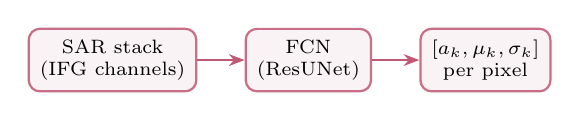
\begin{tikzpicture}[node distance=6mm]
    \node[box] (in)  {SAR stack\\(IFG channels)};
    \node[box, right=of in] (net) {FCN\\(ResUNet)};
    \node[box, right=of net] (out) {$[a_k,\mu_k,\sigma_k]$\\per pixel};
    \draw[flow] (in) -- (net);
    \draw[flow] (net) -- (out);
  \end{tikzpicture}
  \\[2pt]
  {\scriptsize Amortise per-pixel Gaussian-mixture fitting of the elevation spectrum in one forward pass.}
\end{frame}

% ---------------------------------------------------------------- Overview
\begin{frame}{The task}
  \begin{columns}[T]
    \begin{column}{0.56\textwidth}
      \small
      The elevation power spectrum at each pixel is a $K$-Gaussian mixture:
      \[
        p(z)=\sum_{k=1}^{K} a_k\,\exp\!\Big(\!-\tfrac{(z-\mu_k)^2}{2\sigma_k^2}\Big)
      \]
      Classical processing fits this per pixel by nonlinear least squares.
      We train a network to emit all $3K$ parameters directly.
      \[
        f_\theta:\ \mathbb{R}^{C_\text{in}\times P\times P}\ \longrightarrow\ \mathbb{R}^{3K\times P\times P}
      \]
    \end{column}
    \begin{column}{0.44\textwidth}
      \centering
      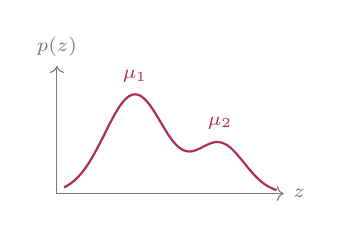
\begin{tikzpicture}[scale=0.9]
        \draw[->,soft] (0,0) -- (3.2,0) node[right,font=\scriptsize]{$z$};
        \draw[->,soft] (0,0) -- (0,1.8) node[above,font=\scriptsize]{$p(z)$};
        \draw[accent,thick,domain=0.1:3.1,samples=60,smooth]
          plot (\x,{1.4*exp(-(\x-1.1)^2/(2*0.18)) + 0.7*exp(-(\x-2.3)^2/(2*0.12))});
        \node[font=\scriptsize,accent] at (1.1,1.65) {$\mu_1$};
        \node[font=\scriptsize,accent] at (2.3,1.0) {$\mu_2$};
      \end{tikzpicture}
      \\[-2pt]
      {\scriptsize Two scatterers at $\mu_1,\mu_2$.}
    \end{column}
  \end{columns}
\end{frame}

% ================================================================ SECTION 1
\begin{frame}[plain]
  \centering \vfill
  {\Large\bfseries\color{accent} 1\ \ Improvements}\\[4pt]
  {\small leaky clamp \; $\cdot$ \; robust normalization \; $\cdot$ \; per-group LR \& warmup}
  \vfill
\end{frame}

% ---- Leaky clamp
\begin{frame}{Improvement --- Output clamp (leaky clamp)}
  \small
  The model predicts in \emph{normalized} space, so the physical bound is enforced by a
  round-trip: denormalize, clamp, renormalize --- the loss is then taken back in normalized space.
  \begin{center}
  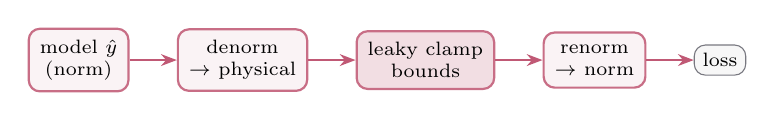
\begin{tikzpicture}[node distance=6mm]
    \node[box] (m)  {model $\hat y$\\{\scriptsize (norm)}};
    \node[box, right=of m] (d) {denorm\\{\scriptsize $\to$ physical}};
    \node[box, fill=accent!16, right=of d] (c) {leaky clamp\\{\scriptsize bounds}};
    \node[box, right=of c] (r) {renorm\\{\scriptsize $\to$ norm}};
    \node[gate, right=of r] (l) {loss};
    \draw[flow] (m)--(d); \draw[flow] (d)--(c); \draw[flow] (c)--(r); \draw[flow] (r)--(l);
  \end{tikzpicture}
  \end{center}
  \begin{columns}[T]
    \begin{column}{0.54\textwidth}
      A saturated head must still receive a gradient toward the valid range:
      \[
        \boxed{\ \tilde x = \mathrm{clamp}(x)\; +\; \lambda\,\big(x-\mathrm{clamp}(x)\big).\text{detach()}\ }
      \]
      \begin{itemize}\scriptsize
        \item Forward $=$ hard clamp; a fraction $\lambda=0.01$ of the residual leaks gradient (straight-through).
        \item Physical bounds: $a\!\in\![0,a_{\max}]$, $\mu\!\in\![x_{\min},x_{\max}]$,
              $\sigma\!\in\![\tfrac12 x_\text{step},\tfrac12 x_\text{range}]$.
        \item Inference uses $\lambda=0$ (plain hard clamp).
      \end{itemize}
    \end{column}
    \begin{column}{0.46\textwidth}
      \centering
      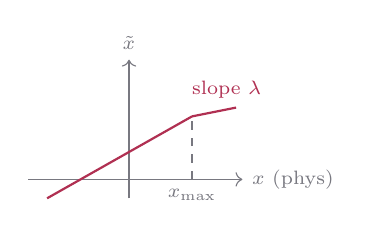
\begin{tikzpicture}[scale=0.8]
        \draw[->,soft] (-1.6,0) -- (1.8,0) node[right,font=\scriptsize]{$x$ (phys)};
        \draw[->,soft] (0,-0.3) -- (0,1.9) node[above,font=\scriptsize]{$\tilde x$};
        \draw[dashed,soft] (1,0) -- (1,1); \node[font=\scriptsize,soft] at (1,-0.25){$x_{\max}$};
        \draw[accent,thick] (-1.3,-0.3) -- (1,1);
        \draw[accent,thick] (1,1) -- (1.7,1.14);
        \node[font=\scriptsize,accent] at (1.55,1.42){slope $\lambda$};
      \end{tikzpicture}
      \\[-2pt]
      {\scriptsize Gradient never fully zero past the bound.}
    \end{column}
  \end{columns}
\end{frame}

% ---- Normalization
\begin{frame}{Improvement --- Robust (IQR) normalization}
  \begin{columns}[T]
    \begin{column}{0.56\textwidth}
      \small
      Heavy-tailed channels switched from z-score to \emph{robust} scaling:
      \[
        \hat x=\frac{x-\mathrm{median}(x)}{\mathrm{IQR}(x)},\qquad
        \mathrm{IQR}=Q_3-Q_1
      \]
      \begin{itemize}\scriptsize
        \item Median / IQR ignore the tails, so rare bright scatterers no
              longer inflate the scale ($+12..+39\sigma$ under z-score).
        \item Applied to \texttt{mag}, \texttt{amp}, \texttt{sigma}, \texttt{dem}
              (with \texttt{log1p} first); \texttt{mu} stays z-score.
        \item Stats pooled over \emph{active} pixels only ($a>10^{-2}$).
      \end{itemize}
    \end{column}
    \begin{column}{0.44\textwidth}
      \centering
      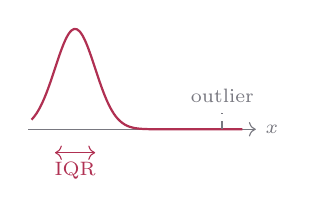
\begin{tikzpicture}[scale=0.85]
        \draw[->,soft] (0,0)--(3.4,0) node[right,font=\scriptsize]{$x$};
        \draw[accent,thick,domain=0.05:3.2,samples=80,smooth]
          plot (\x,{1.5*exp(-(\x-0.7)^2/(2*0.09))});
        \draw[soft,thick,dashed] (2.9,0)--(2.9,0.25);
        \node[font=\scriptsize,soft] at (2.9,0.5){outlier};
        \draw[<->,accent] (0.4,-0.35)--(1.0,-0.35) node[midway,below,font=\scriptsize]{IQR};
      \end{tikzpicture}
      \\[-2pt]
      {\scriptsize Scale set by the bulk, not the tail.}
    \end{column}
  \end{columns}
\end{frame}

% ---- LR
\begin{frame}{Improvement --- Per-group LR + warmup}
  \small
  Each submodule gets its own base LR; a step-level warmup ramps in, and a cosine
  schedule anneals per epoch:
  \[
    \boxed{\ \eta_\text{eff}=\eta_0\cdot \underbrace{F(t)}_{\text{cosine}}\cdot
      \underbrace{f_\text{warm}(s)}_{\text{ramp}}\ }\qquad
    f_\text{warm}(s)=\alpha_0+(1-\alpha_0)\tfrac{s}{S}
  \]
  \begin{columns}[T]
    \begin{column}{0.5\textwidth}
      \begin{itemize}\scriptsize
        \item Groups: encoder / decoder $=3\!\times\!10^{-4}$, output head $=10^{-3}$ (head learns faster).
        \item Warmup: $S=200$ steps, start $\alpha_0=0.1$; cosine floor $\eta_{\min}=10^{-6}$.
        \item LR auto-scales with batch size.
      \end{itemize}
    \end{column}
    \begin{column}{0.5\textwidth}
      \centering
      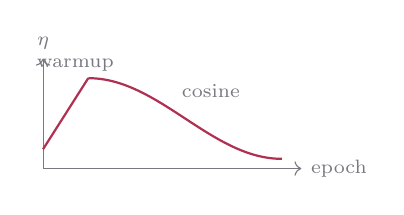
\begin{tikzpicture}[scale=0.82]
        \draw[->,soft] (0,0)--(4,0) node[right,font=\scriptsize]{epoch};
        \draw[->,soft] (0,0)--(0,1.7) node[above,font=\scriptsize]{$\eta$};
        % warmup ramp
        \draw[accent,thick] (0,0.3)--(0.7,1.4);
        % cosine decay
        \draw[accent,thick,domain=0.7:3.7,samples=50,smooth]
          plot (\x,{0.15+1.25*0.5*(1+cos(deg((\x-0.7)/3*pi)))});
        \node[font=\scriptsize,soft] at (0.5,1.6){warmup};
        \node[font=\scriptsize,soft] at (2.6,1.2){cosine};
      \end{tikzpicture}
    \end{column}
  \end{columns}
\end{frame}

% ================================================================ SECTION 2
\begin{frame}[plain]
  \centering \vfill
  {\Large\bfseries\color{accent} 2\ \ Additions}\\[4pt]
  {\small augmentation \; $\cdot$ \; Hungarian matching \; $\cdot$ \; model $\times$ loss benchmark}
  \vfill
\end{frame}

% ---- Augmentation + Hungarian
\begin{frame}{Addition --- Augmentation \& Hungarian matching}
  \begin{columns}[T]
    \begin{column}{0.48\textwidth}
      \small\textbf{Augmentation}
      \begin{itemize}\scriptsize
        \item Joint H/V flips ($p=0.5$) on input+target (keeps spatial correspondence).
        \item Optional $90^\circ$ rotation (off by default; skipped when geometry present).
        \item Input-only Gaussian noise, in normalized units.
      \end{itemize}
      \vspace{2pt}
      \centering
      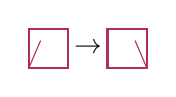
\begin{tikzpicture}[scale=0.5]
        \draw[accent,thick] (0,0) rectangle (1,1); \draw[accent] (0,0)--(0.3,0.7);
        \node at (1.5,0.5){$\to$};
        \draw[accent,thick] (2,0) rectangle (3,1); \draw[accent] (3,0)--(2.7,0.7);
      \end{tikzpicture}
    \end{column}
    \begin{column}{0.52\textwidth}
      \small\textbf{Hungarian matching}
      \[
        \pi^\star=\arg\min_{\pi\in S_K}\sum_{k} w_k\,\big\|\,\hat p_k - p_{\pi(k)}\big\|_1
      \]
      \begin{itemize}\scriptsize
        \item Default training matcher: permutation-invariant slot alignment.
        \item Brute-force over $K!$ perms ($K\!\le\!6$), vectorised over pixels
              (\emph{not} \texttt{scipy}); inactive GT slots excluded.
        \item Removes the ``Gaussian $k$ in slot $k$'' constraint.
      \end{itemize}
    \end{column}
  \end{columns}
\end{frame}

% ---- Class imbalance
\begin{frame}{Addition --- Slot rebalancing (ships with Hungarian)}
  \small
  \begin{columns}[T]
    \begin{column}{0.5\textwidth}
      \textbf{Active normalization}\\
      Reduce the parameter loss as a weighted mean over \emph{active} slots only:
      \[
        \mathcal{L}=\frac{\sum_k m_k\,\ell_k}{\sum_k m_k},\quad m_k=\mathbb{1}[a_k^\text{GT}\!>\!\tau]
      \]
      {\scriptsize Empty slots (GT mean $\approx1.28$ of $6$) stop diluting the gradient.}
    \end{column}
    \begin{column}{0.5\textwidth}
      \textbf{Presence balance}\\
      Inverse-frequency reweighting of the amplitude term, per batch:
      \[
        w_\text{act}=\frac{1}{\rho},\quad w_\text{inact}=\frac{1}{1-\rho},\quad
        \rho=\tfrac{\#\text{active}}{\#\text{slots}}
      \]
      {\scriptsize Under-represented active Gaussians get up-weighted automatically.}
    \end{column}
  \end{columns}
  \vspace{4pt}
  \begin{center}\scriptsize
  These two are the full model's only slot-presence terms --- \emph{no} presence head, BCE, or focal.
  \end{center}
  \vspace{2pt}
  \begin{block}{}\scriptsize
    \textbf{When to use it:} Hungarian + balance is a \emph{high-$K$} strategy --- it pays off
    when many Gaussians compete for slots. At $K=2$ the simpler \texttt{sort\_gt\_by\_mu}
    matching wins, so it stays the default there.
  \end{block}
\end{frame}

% ---- Benchmark
\begin{frame}{Addition --- Model $\times$ loss benchmark}
  \begin{columns}[T]
    \begin{column}{0.5\textwidth}
      \small
      Capacity-matched sweep: 10 architectures at $\approx\!30$M params, identical recipe,
      each $\times$ several loss components.
      \begin{center}
      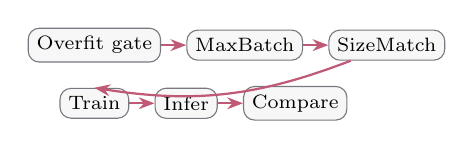
\begin{tikzpicture}[node distance=3.2mm]
        \node[gate](a){Overfit gate};
        \node[gate,right=of a](b){MaxBatch};
        \node[gate,right=of b](c){SizeMatch};
        \draw[flow](a)--(b); \draw[flow](b)--(c);
        \node[gate,below=3.2mm of a](d){Train};
        \node[gate,right=of d](e){Infer};
        \node[gate,right=of e](f){Compare};
        \draw[flow](d)--(e); \draw[flow](e)--(f);
        \draw[flow](c) to[bend left=15] (d.north);
      \end{tikzpicture}
      \end{center}
    \end{column}
    \begin{column}{0.5\textwidth}
      \centering \scriptsize
      \textbf{Curve-level $R^2$ (top of field)}\\[2pt]
      \begin{tabular}{lc}
        \toprule
        Model & $R^2$ \\
        \midrule
        \textbf{resunet} & \textbf{0.593} \\
        unet++           & 0.555 \\
        attention\_unet  & 0.542 \\
        unet             & 0.530 \\
        transunet / unetr& $\approx$0.42 \\
        \bottomrule
      \end{tabular}
      \\[3pt]
      CNN U-Nets lead; transformer hybrids trail at matched capacity.
    \end{column}
  \end{columns}
\end{frame}

% ================================================================ SECTION 3
\begin{frame}[plain]
  \centering \vfill
  {\Large\bfseries\color{accent} 3\ \ Future}\\[4pt]
  {\small loss curriculum \; $\cdot$ \; physical (SAR) loss terms}
  \vfill
\end{frame}

% ---- Curriculum
\begin{frame}{Future --- Loss curriculum}
  \small
  Warm up with a simple loss, then swap to the full composite at a fixed epoch,
  optionally resetting the schedule, warmup, and Adam moments.
  \begin{center}
  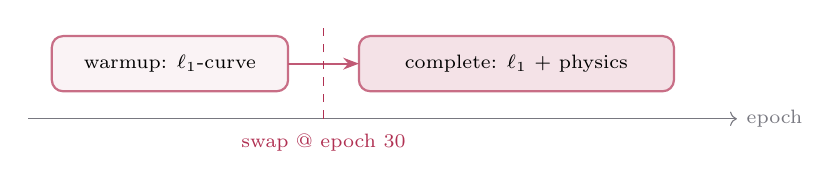
\begin{tikzpicture}
    \draw[->,soft] (0,0)--(9,0) node[right,font=\scriptsize]{epoch};
    \node[box,minimum width=3cm] (w) at (1.8,0.7) {\scriptsize warmup: $\ell_1$-curve};
    \node[box,minimum width=4cm,fill=accent!14] (c) at (6.2,0.7) {\scriptsize complete: $\ell_1$ + physics};
    \draw[flow] (3.3,0.7) -- (4.2,0.7);
    \draw[dashed,accent] (3.75,0)--(3.75,1.15);
    \node[font=\scriptsize,accent] at (3.75,-0.3){swap @ epoch 30};
  \end{tikzpicture}
  \end{center}
  \begin{itemize}\scriptsize
    \item Both phases use Hungarian matching + active-norm + presence-balance.
    \item Checkpoint baseline auto-resets across the (non-comparable) loss scale.
  \end{itemize}
\end{frame}

% ---- Physics loss
\begin{frame}{Future --- Physical (SAR) loss terms}
  \small
  Match the predicted reflectivity to the observed interferometric covariance via the
  steering operator, rather than only in parameter space:
  \[
    \hat R_{ij}=\int p(z)\,e^{\,j(k_{z,i}-k_{z,j})z}\,dz,\qquad
    k_z=\frac{4\pi\,b_\perp}{\lambda\,r_0}
  \]
  \[
    \mathcal{L}_\text{phys}=\big\|\hat R(\hat p)-\hat R(p^\text{GT})\big\|_F^2
  \]
  \begin{columns}[T]
    \begin{column}{0.58\textwidth}
      \begin{itemize}\scriptsize
        \item Ranked: (1) covariance matching, (2) coherence re-synthesis; moments as a metric.
        \item $k_z$ from perpendicular baselines; steering sign settled ($+k_z$, $0.67$m median peak error).
        \item \texttt{total\_power} rejected as a loss (Capon $\sim$2\,dB scene bias).
      \end{itemize}
    \end{column}
    \begin{column}{0.42\textwidth}
      \centering
      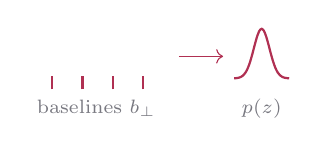
\begin{tikzpicture}[scale=0.7]
        \foreach \i in {0,1,2,3} \draw[accent,thick] (\i*0.55,0)--(\i*0.55,0.25);
        \node[soft,font=\scriptsize] at (0.8,-0.35){baselines $b_\perp$};
        \draw[->,accent] (2.3,0.6)--(3.1,0.6);
        \draw[accent,thick,domain=0:1,samples=25,smooth] plot ({3.3+\x},{0.2+0.9*exp(-(\x-0.5)^2/0.04)});
        \node[soft,font=\scriptsize] at (3.8,-0.35){$p(z)$};
      \end{tikzpicture}
    \end{column}
  \end{columns}
\end{frame}

% ================================================================ SECTION 4
\begin{frame}[plain]
  \centering \vfill
  {\Large\bfseries\color{accent} 4\ \ Results}\\[4pt]
  {\small 16 architectures \; $\times$ \; 6 loss functions \; $\cdot$ \; 96 runs \; $\cdot$ \; curve-level $R^2$}
  \vfill
\end{frame}

% ---- Results: design
\begin{frame}{Result --- Benchmark design}
  \small
  A joint \textbf{architecture $\times$ loss} sweep: \textbf{16 architectures} each trained
  under \textbf{6 loss functions} (\textbf{96 runs}), all capacity-matched to $\approx\!30$M
  parameters under one identical recipe and passed through the same staged gates --- so each
  cell isolates the architecture $\times$ loss pairing.
  \begin{columns}[T]
    \begin{column}{0.55\textwidth}
      \textbf{\scriptsize 16 architectures}\\[1pt]
      {\scriptsize single-head backbones only (the multi-head / per-Gaussian variants and
      \texttt{unet\_skip} are excluded):}
      \begin{itemize}\scriptsize
        \item unet, resunet, attention\_unet, unet++, linknet
        \item swin\_unet, transunet, unetr, deeplabv3+, segformer
        \item convnext\_unet, dense\_unet, hrnet
        \item multires\_unet, fpn, u2net
      \end{itemize}
    \end{column}
    \begin{column}{0.45\textwidth}
      \centering\scriptsize
      \textbf{6 loss functions}\\[2pt]
      \begin{tabular}{lcc}
        \toprule
        Loss & Kind & Space \\
        \midrule
        \texttt{l1\_curve}          & L1     & curve \\
        \texttt{mse\_curve}         & MSE    & curve \\
        \texttt{param\_l1}          & L1     & param \\
        \texttt{param\_mse}         & MSE    & param \\
        \texttt{charbonnier\_curve} & Charb. & curve \\
        \texttt{cosine\_curve}      & cosine & curve \\
        \bottomrule
      \end{tabular}
      \\[3pt]
      {\scriptsize L1 \& MSE in both spaces, plus Charbonnier and cosine.}
    \end{column}
  \end{columns}
\end{frame}

% ---- Results: grid
\begin{frame}{Result --- Curve-level $R^2$ grid}
  \centering \tiny
  \setlength{\tabcolsep}{4pt}\renewcommand{\arraystretch}{1.18}
  \begin{tabular}{lcccccc}
    \toprule
    Model & L1$_\text{c}$ & MSE$_\text{c}$ & L1$_\text{p}$ & MSE$_\text{p}$ & Charb & Cos \\
    \midrule
    unet            & -- & -- & -- & -- & -- & -- \\
    resunet         & -- & -- & -- & -- & -- & -- \\
    attention\_unet & -- & -- & -- & -- & -- & -- \\
    unet++          & -- & -- & -- & -- & -- & -- \\
    linknet         & -- & -- & -- & -- & -- & -- \\
    swin\_unet      & -- & -- & -- & -- & -- & -- \\
    transunet       & -- & -- & -- & -- & -- & -- \\
    unetr           & -- & -- & -- & -- & -- & -- \\
    deeplabv3+      & -- & -- & -- & -- & -- & -- \\
    segformer       & -- & -- & -- & -- & -- & -- \\
    convnext\_unet  & -- & -- & -- & -- & -- & -- \\
    dense\_unet     & -- & -- & -- & -- & -- & -- \\
    hrnet           & -- & -- & -- & -- & -- & -- \\
    multires\_unet  & -- & -- & -- & -- & -- & -- \\
    fpn             & -- & -- & -- & -- & -- & -- \\
    u2net           & -- & -- & -- & -- & -- & -- \\
    \bottomrule
  \end{tabular}
  \\[4pt]
  {\scriptsize Curve-level $R^2$ on the held-out test split (higher is better); best cell to
  be highlighted. \emph{Numbers to be filled from the benchmark run.}}
\end{frame}

% ---------------------------------------------------------------- Close
\begin{frame}[plain]
  \centering\vfill
  {\large\bfseries\color{accent} Summary}\\[6pt]
  \small
  \begin{tabular}{ll}
    \textbf{Improvements} & leaky clamp $\cdot$ IQR norm $\cdot$ per-group LR + warmup \\[2pt]
    \textbf{Additions}    & augmentation $\cdot$ Hungarian + rebalancing $\cdot$ benchmark \\[2pt]
    \textbf{Future}       & loss curriculum $\cdot$ physical SAR loss \\[2pt]
    \textbf{Results}      & 16 architectures $\times$ 6 losses $\cdot$ curve-level $R^2$ grid \\
  \end{tabular}
  \vfill
\end{frame}

\end{document}
